%!TEX root = ./exercice2.tex

\section{Identification of a Laser Beam Stabilizing System}
The following section explains identification algorithms using data from the laser beam stabilizing system shown in Figure~\ref{fig:system}.
We have access to time-domain data in the file \texttt{laserbeamdataN.mat}.
This file contains the input $u$ and the output signal $y$ of the laser beam stabilizing system and has $N=500$ samples.

\begin{figure}[h]
	\centering
	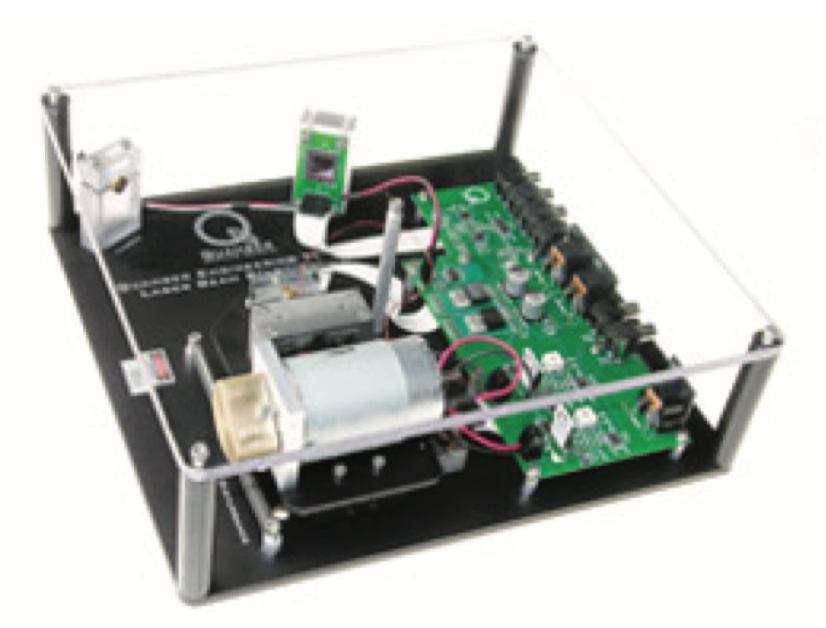
\includegraphics[height=4cm]{figures/system.png}
	\caption{Laser beam stabilizing system }\label{fig:system}
\end{figure}

\subsection{FIR Model Identification}\label{sec:FIR}
In this section we identify a finite impulse response (FIR) model of the form
\begin{equation}\label{eq:FIRmodel}
	\hat{y}(k,\theta) = b_1 u(k-1) + \cdots + b_m u(k-m) \qquad m = 1,2,\ldots,50 \, ,
\end{equation}
which can be rewritten to
\begin{align}\label{eq:FIRrewritten}
	 \hat{y} (k,\theta) & = \phi^{T} (k) \theta 
 \intertext{where}
 	 \phi^{T} (k) & = \left[ u(k-1), u(k-2), \ldots, u(k-m) \right] \\
 	 \theta^T & = \left[ b_1, b_2, \ldots, b_m \right] .
\end{align}

First, we compute the parameter vector $\hat{\theta}$ using the least squares algorithm and the Moore-Penrose pseudo inverse $\pmb{\phi}^+$ of $\pmb{\phi}$
\begin{equation}\label{eq:FIRmodel}
	\hat{\theta} = \left[ \sum\limits_{k=1}^N \phi(k)\phi^T(k) \right]^{-1} \sum\limits_{k=1}^N 
\phi(k) y(k) = \left( \pmb{\phi}^T \pmb{\phi} \right)^{-1} \pmb{\phi}^T \textbf{Y} = \pmb{\phi}^+ \textbf{Y}.
\end{equation}
Here, $\pmb{\phi}$ is an asymmetric (lower) triangular Toeplitz matrix, which we generate with the MATLAB \texttt{toeplitz} command.
In MATLAB we can solve this least squares problem by simply using the backslash operator. 
Afterwards, we compute the predicted output of our identified model $\hat{y} (k,\hat{\theta}) = \phi^{T} (k) \hat{\theta}$. 
The code is shown in Listing~\ref{lst:FIR} (page~\pageref{lst:FIR}) and the result can be seen in Figure~\ref{fig:output_fir}.
\begin{figure}[h]
	\centering
	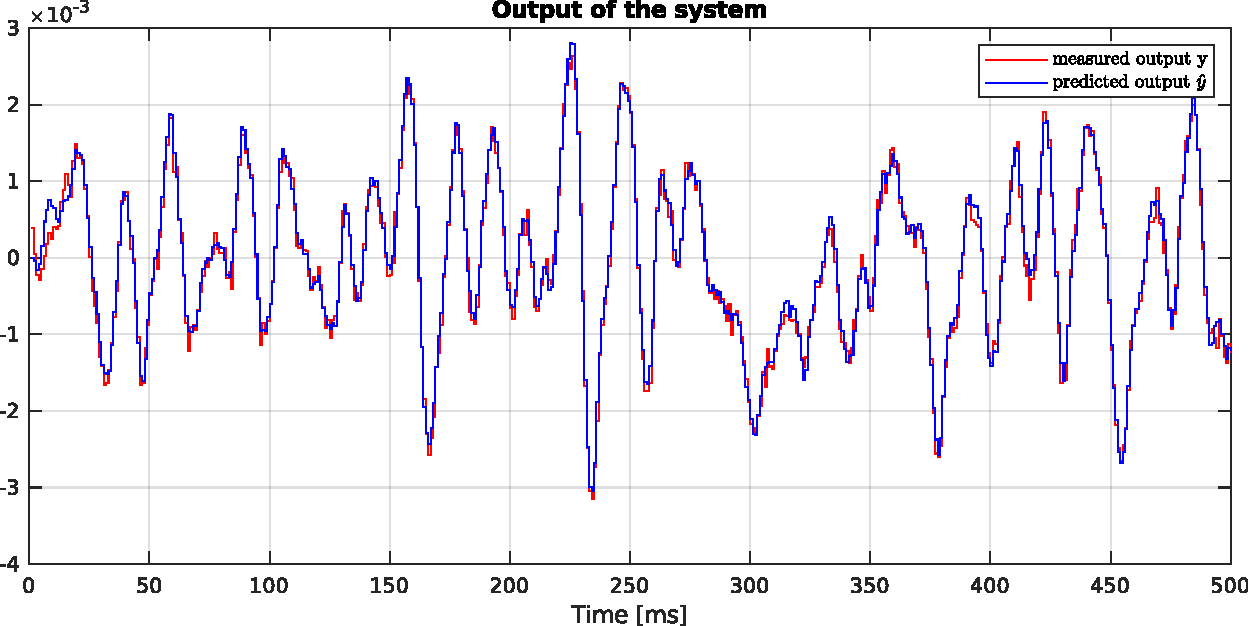
\includegraphics[height=5.5cm]{figures/output.pdf}
	\caption{Predicted and measured output of the system}\label{fig:output_fir}
\end{figure}
In order to estimate the quality of our predictor, we need a fit criterion, which should minimized. We therefore consider the function
\begin{equation}\label{eq:J}
	J(\theta) = \sum\limits_{k=1}^N \left[y(k) - \hat{y}(k,\theta) \right]^2.
\end{equation}
Using the MATLAB command \texttt{norm} and squaring the result we obtain $ J(\theta) \approx 6.92 \cdot 10^{-6}$. 
As we assume that the noise is white, we obtain an unbiased estimate of the noise variance using
\begin{equation}\label{eq:sigma}
	\hat{\sigma}_{noise}^{2} = \frac{1}{N-m} J(\hat{\theta}) .
\end{equation}
Using the available data this equation yields to $ \hat{\sigma}_{noise} \approx 1.24 \cdot 10^{-4} $.
The covariance of the parameter estimates can then be obtained using
\begin{equation}\label{eq:cov}
	cov[\hat{\theta}] = \hat{\sigma}_{noise}^2 \left[ \sum\limits_{k=1}^N \phi(k)\phi^T(k) \right]^{-1} = \hat{\sigma}_{noise}^2 \left( \pmb{\phi}^T \pmb{\phi} \right)^{-1} .
\end{equation}
The square root of the diagonal elements of the $cov[\hat{\theta}]$ matrix is the standard deviation $ \sigma $, which we use for the $ \pm 2 \sigma $ confidence interval in Figure~\ref{fig:fir_response}. This figure shows us the finite impulse response of the system.
\begin{figure}[h]
	\centering
	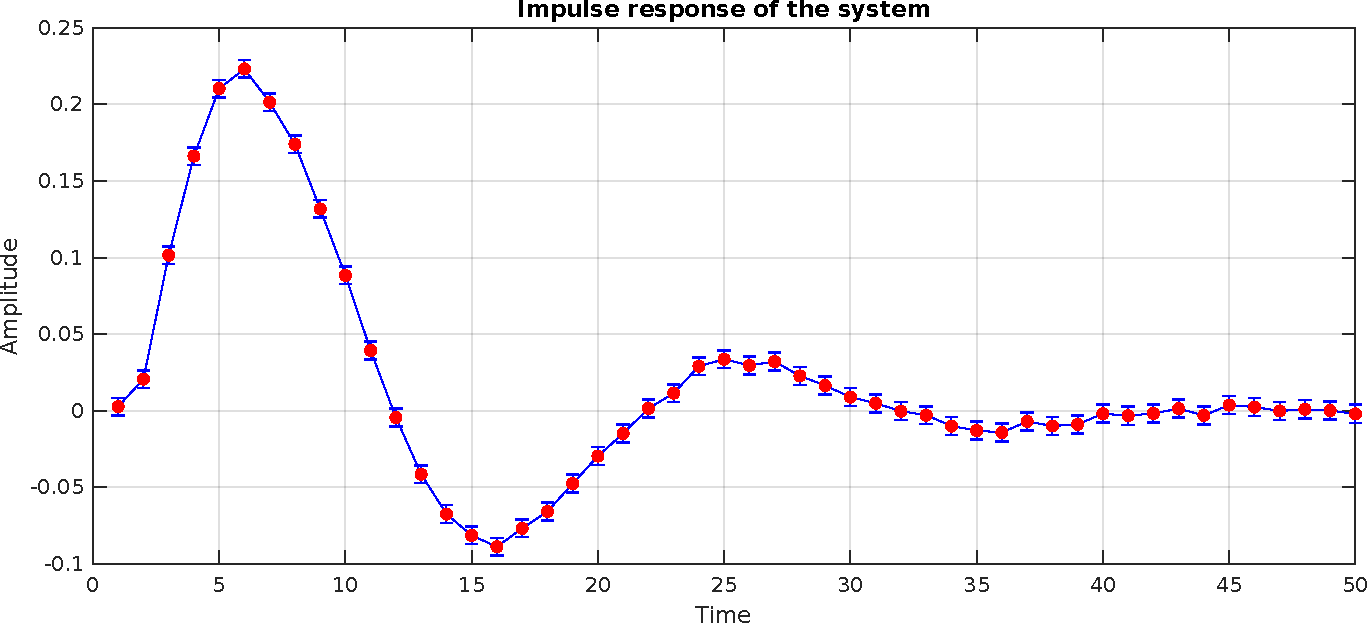
\includegraphics[height=5.5cm]{figures/fir_response.pdf}
	\caption{Identified finite impulse response of the laser beam stabilization system. The error bars show the $2\sigma$ confidence interval of the estimates.}\label{fig:fir_response}
\end{figure}

\subsection{ARX Model Identification}
We now assume a second order auto-regressive with external input (ARX) model for the same data as in the previous section. 
Consequently, we use the following predictor
\begin{align}\label{eq:arx}
	\hat{y}(k,\theta) & = -a_1 y(k-1) - a_2 y(k-2) + b_1 u(k-1) + b_2u (k-2) = \phi^T(k) \theta
	\intertext{where}
 	 \phi^{T} (k) & = \left[ -y(k-1), -y(k-2), u(k-1), u(k-2) \right] \\
 	 \theta^T & = \left[ a_1, a_2, b_1, b_2\right] .
\end{align}
We observe that the system has no modeled delay as $d = 0$.
Using the least squares algorithm and the Moore-Penrose pseudo inverse $\pmb{\phi}^+$ of $\pmb{\phi}$, we compute, like we already did in Section~\ref{sec:FIR}, the parameter vector $\hat{\theta}$ according to
\begin{equation}\label{eq:ARXmodel}
	\hat{\theta} = \left[ \sum\limits_{k=1}^N \phi(k)\phi^T(k) \right]^{-1} \sum\limits_{k=1}^N 
\phi(k) y(k) = \left( \pmb{\phi}^T \pmb{\phi} \right)^{-1} \pmb{\phi}^T \textbf{Y} = \pmb{\phi}^+ \textbf{Y}.
\end{equation}
We construct the matrix consisting of the input and output values according to the predictor structure and solve for the parameters using the backlash operator.
Listing~\ref{lst:ARX} on page~\pageref{lst:ARX} shows the implementation in MATLAB.
The predicted output of our identified model $\hat{y}(k,\hat{\theta})$ is then computed using $\hat{y}(k,\hat{\theta}) = \phi^{T} (k) \hat{\theta}$. 
The result can be seen in Figure~\ref{fig:output_arx}.
Note that this predictor (in contrast to the simulated transfer function below) uses the measured past value of the output.
In order to estimate the quality of our predictor, we need a fit criterion, which should be minimized. Hence, we consider a loss function as 
\begin{equation}\label{eq:J}
	J(\theta) = \sum\limits_{k=1}^N \left[y(k) - \hat{y}(k,\theta) \right]^2.
\end{equation}
Using this, we obtain $ J(\theta) \approx 2.17 \cdot 10^{-5}$. 
Afterwards we compute the output of the identified model $y_m(k)$ using the MATLAB command \texttt{lsim} and the transfer function of the model
\begin{equation}
	G_0(q) = \frac{b_1 q^{-1} + b_2 q^{-2}}{1 + a_1 q^{-1} + a_2 q^{-2}}
	= \frac{0.0183q^{-1} + 0.0731q^{-2}}{1 - 1.5483q^{-1} + 0.6484q^{-2}}\, .
\end{equation}
We generate a transfer function object using the MATLAB command \texttt{tf} and simulate the output given the input $u(k)$ and we plot the simulated output resulting from the second order model with the measured output in Figure~\ref{fig:output_lsim2}.
The resulting sum of the squares of the error is then $ J_{tf}(\hat{\theta}) \approx 1.14 \cdot 10^{-4}$. 
\begin{figure}[h!]
	\centering
	\begin{subfigure}{.49\textwidth}
		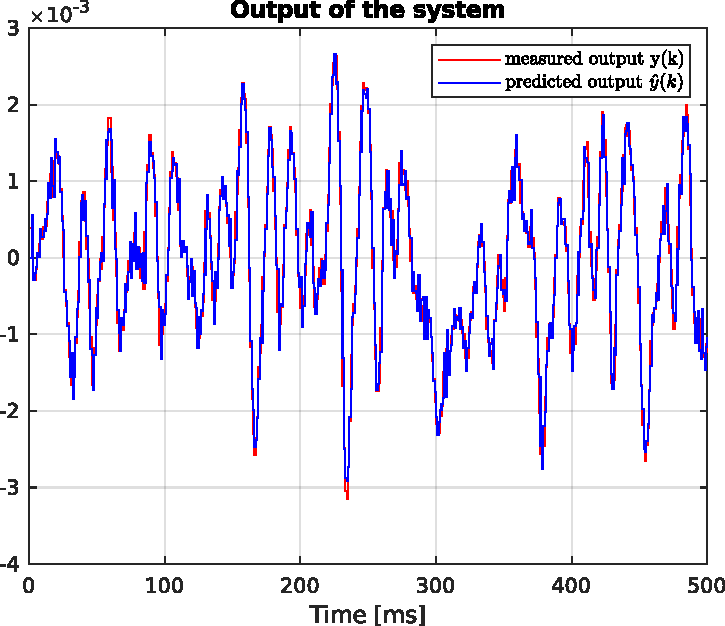
\includegraphics[width=\textwidth]{figures/output_arx.pdf}
		\subcaption{Comparison of measured output $y$ and predicted output $\hat{y}$ using the past measured output.}\label{fig:output_arx}
	\end{subfigure}\hfill
	\begin{subfigure}{.49\textwidth}
		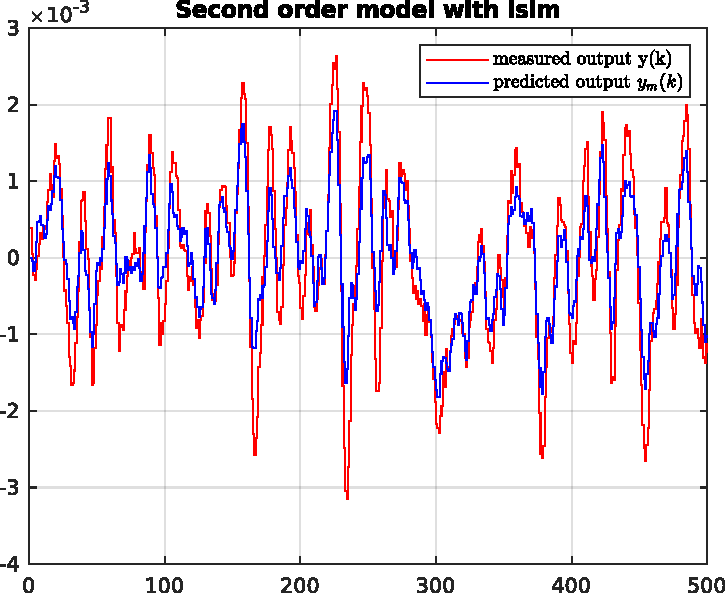
\includegraphics[width=\textwidth]{figures/output_lsim2.pdf}
		\subcaption{Comparison of measured output $y$ and predicted output $y_m$ using only the input and a transfer function model.}\label{fig:output_lsim2}
	\end{subfigure}
	\begin{subfigure}{\textwidth}
		\vspace*{1cm}
		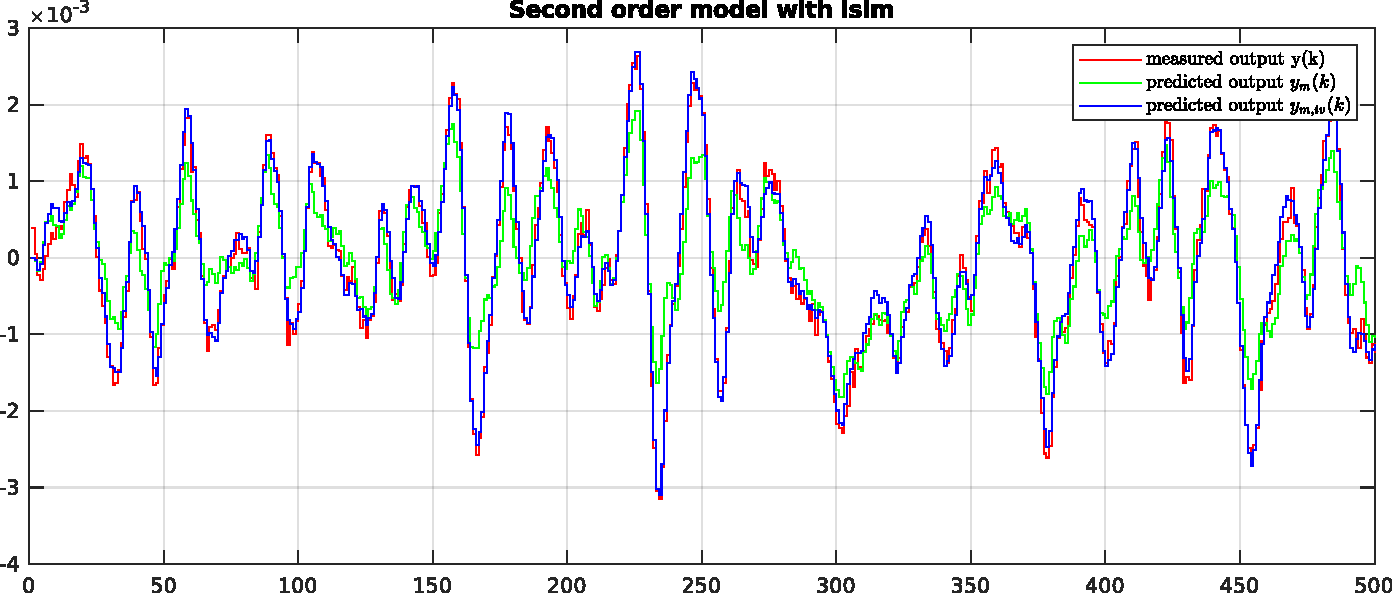
\includegraphics[width=\textwidth]{figures/arx_iv.pdf}
		\subcaption{Comparison of the measured output and the predicted output. The simulated output is shown for the model parametrized by the parameters identified using the plain ARX method and the IV method with $4$ iterations, respectively.} \label{fig:output_arx_iv}
	\end{subfigure}
	\caption{Comparison of predicted and measured output. Upper part: comparison with predictor using the past measured output and comparison only using the input data and the simulated transfer function model. Lower part:comparison of ARX model with IV method and past measured output}
\end{figure}
In order to obtain unbiased estimates the following two conditions must be satisfied: 
\begin{enumerate}
\item $R_{\phi \phi}$ is not singular,
\item $R_{\phi e }(0) = 0$.
\end{enumerate}
These conditions can be satisfied by replacing the non-transposed $\phi$'s in the estimator for $\hat{\theta}$ by a new vector $\phi_{iv}$ called the vector of  instrumental variables (IV):
\begin{equation}
	\hat{\theta}_{iv} = \left[ \sum\limits_{k=1}^N \phi_{iv}(k)\phi^T(k) \right]^{-1} \left[\sum\limits_{k=1}^N \phi_{iv}(k) y(k) \right]
\end{equation}
Therefore, the estimates are asymptotically unbiased, if 
\begin{enumerate}
	\item $R_{\phi_{iv} \phi}$ is not singular,
	\item $R_{\phi_{iv} e }(0) = 0$.
\end{enumerate}
That means, choosing an vector of instrumental variables, that is correlated with the regressor vector $\phi$ and uncorrelated with the noise $e$ leads to asymptotically unbiased estimates.
One choice of this vector is keeping the past, non-noisy inputs in the vector and replacing the past noisy outputs using the output of an already identified model $M(q^{-1})$. A noiseless output of this model can be computed by 
\begin{equation}
y_m(k) = M(q^{-1}) u(k)
\end{equation}
and the vector $\phi_{iv}$ is defined as
\begin{equation}
\phi_{iv}^T(k) = \left[-y_M(k-1),\ldots,-y_M(k-n),u(k-d-1),\ldots,u(k-d-m)\right]
\end{equation}
with $d=0$. 
Therefore, we can first identify an ARX model without the use of instrumental variables. 
Afterwards, we use the identified parameters as instrumental variables and repeat the ARX fitting.
In order to obtain better results, this process can be repeated for several iterations. 
For a good trade off between computational cost and accuracy, we choose an IV method with $4$ iterations. 
The resulting parameter vector is $\hat{\theta}_{iv}^T = \left[-1.756, 0.8518, 0.0174, 0.0688\right]$.
The result of the instrumental variables method compared to the measured output and the predicted output of the transfer function model can be seen in Figure~\ref{fig:output_arx_iv} and the implementation can be viewed, again, in Listing~\ref{lst:ARX} (page~\pageref{lst:ARX}).
Note that the function performs ARX identification with and without the IV method.
Setting \texttt{iterations} to 1 means that no IV method is used.
We can observe, that the predicted output of the model identified using the IV method is closer to the measured output.

\subsection{State-space Model Identification}
In this part, a state-space model for the laser beam stabilizing system using the subspace method based on the extended observability matrix is identified. \\
First, the following matrices are defined: 
\begin{align}
 Y &= \left[Y_r(1), Y_r(2),\ldots,Y_r(N) \right] \\
 U &= \left[U_r(1), U_r(2),\ldots,U_r(N) \right] \\
 X &= \left[x_r(1), x_r(2),\ldots,x_r(N) \right]
\end{align}
with 
\quad $Y_r(k) = \left[ \begin{array}{c} y(k) \\\ y(k+1) \\\ \vdots \\\ y(k + r -1) \end{array}\right] $ , \quad $U_r(k) = \left[ \begin{array}{c} u(k) \\\ u(k+1) \\\ \vdots \\\ u(k + r -1) \end{array}\right] $ \quad and \quad $r > n $.\\
The output of the noise-free state-space model can be written as
\begin{equation}
y(k+i) = CA^{i}x(k) + CA^{i-1}Bu(k) + CA^{i-2}Bu(k+1) + \cdots + CBu(k+i-1) + Du(k+i)
\end{equation}
and as 
\begin{equation}
\textbf{Y} = O_r \textbf{X} + S_r \textbf{U}
\label{eq:statespace}
\end{equation}
respectively. 
To get rid of the unknown matrix $S_r$ the following $ N \times N $ matrix is formed: 
\begin{equation}
\textbf{U}^{\bot} = \textbf{I} - \textbf{U}^{T}(\textbf{U}\textbf{U}^{T})^{-1}\textbf{U} \quad \text{with} \quad \textbf{U}\textbf{U}^{\bot} = 0.
\end{equation}
By multiplying Equation~\ref{eq:statespace} with $\textbf{U}^{\bot}$ from the right, we obtain:
\begin{equation}
	Q = \textbf{Y}\textbf{U}^{\bot} = O_r\textbf{X}\textbf{U}^{\bot}.
\end{equation}
Afterwards, we compute the singular values of $Q$ with the MATLAB command \texttt{svd}. 
Using the singular values of the matrix, we determine the model order by choosing the smallest $n \le r$ such that
\begin{equation}
	\sum\limits_{k=0}^{n}\sigma_k \ge 0.8\sum\limits_{k=0}^{r}\sigma_k\, ,
\end{equation}
i.e. we select the smallest model order $n$ such that the first $n$ singular values sum up to at least $0.8$ of the total sum of the singular values.
Here, we get a model order of $n = 3$.
The singular values of $Q$ can be seen in Figure~\ref{fig:singular}. 

\begin{figure}[h]
	\centering
	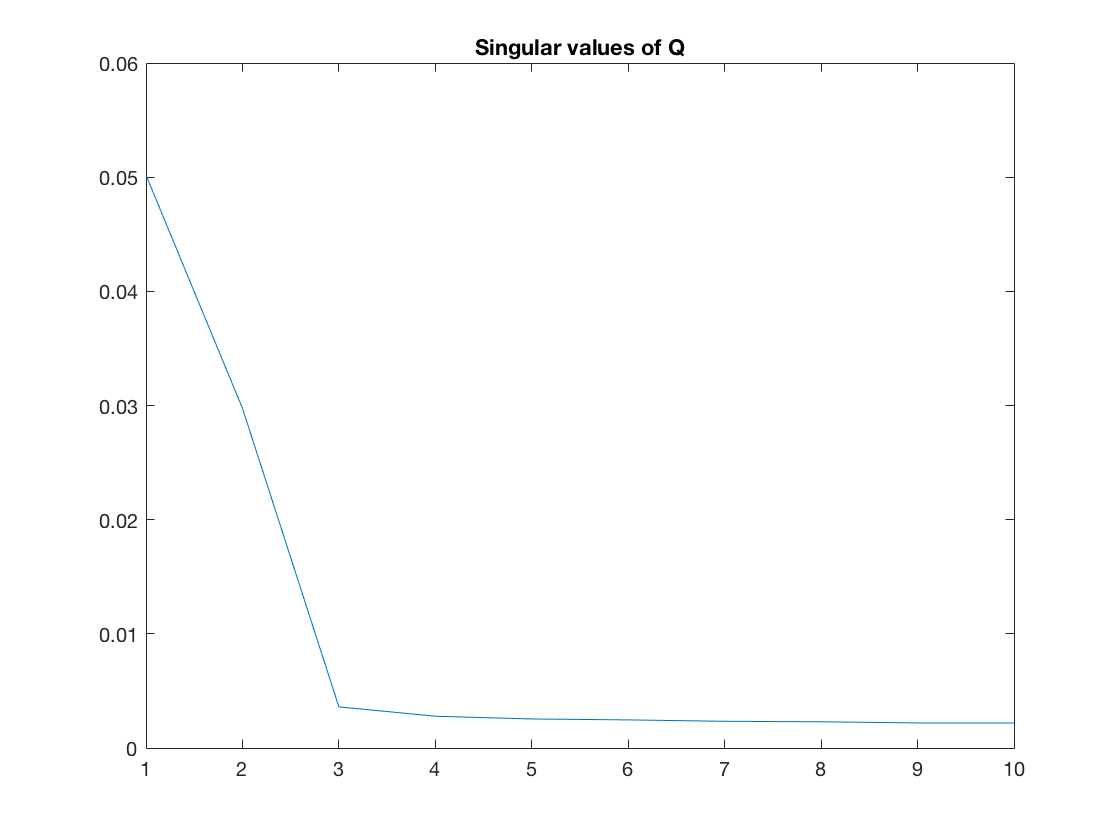
\includegraphics[height=7cm]{figures/singular.png}
	\caption{Singular values of $Q$}\label{fig:singular}
\end{figure}


Then, based on the model order, the matrices for the states space model are computed as provided in the course notes.
The code is shown in Listing~\ref{lst:ss_id} (page~\pageref{lst:ss_id}).
We get the following solutions
\begin{eqnarray}
	\mathbf{A} &=& \begin{bmatrix}
			-0.0645  & 0.0415 & -0.5397\\
			 0.7140  & 0.2319 &  0.1857\\
			-0.3840  & 1.2511 &  0.8986\\
	\end{bmatrix}\,,\\
	\mathbf{B} &=& \begin{bmatrix}
		 -41.5124\\
		-165.7229\\
		-105.1717\\
	\end{bmatrix}\,,\\
	\mathbf{C} &=& 10^{-3} \cdot \begin{bmatrix}
	    0.3697 & -0.0396 & -0.2972
	\end{bmatrix}\, ,\\
	\mathbf{D} &=& 0\, .
\end{eqnarray}

Figure~\ref{fig:ss_id_results} shows the results of the simulation of the identified state-space model using the input data $u$.
We get a residual loss of $J(\theta) = 8.23 \cdot 10^{-6}$.

\begin{figure}[h]
	\begin{subfigure}{0.49\textwidth}
		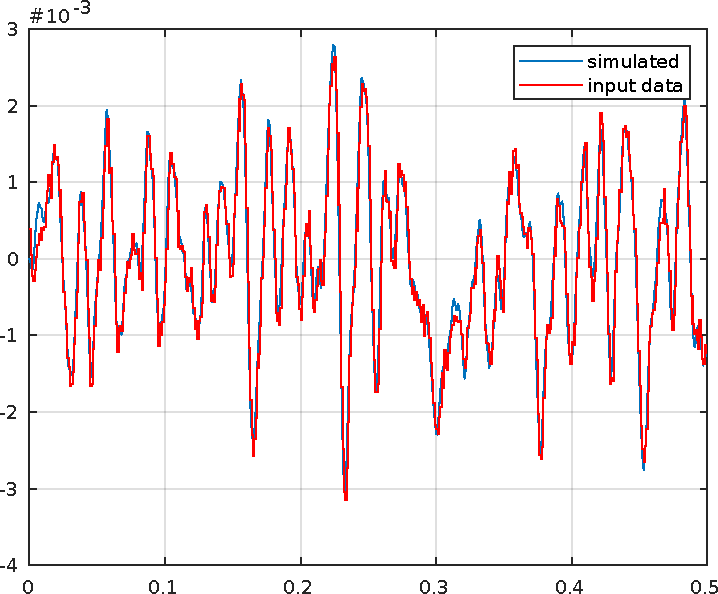
\includegraphics[width=\textwidth]{figures/ss_id_output.pdf}	
		\subcaption{Comparison of outputs}
	\end{subfigure}
	\begin{subfigure}{0.49\textwidth}
		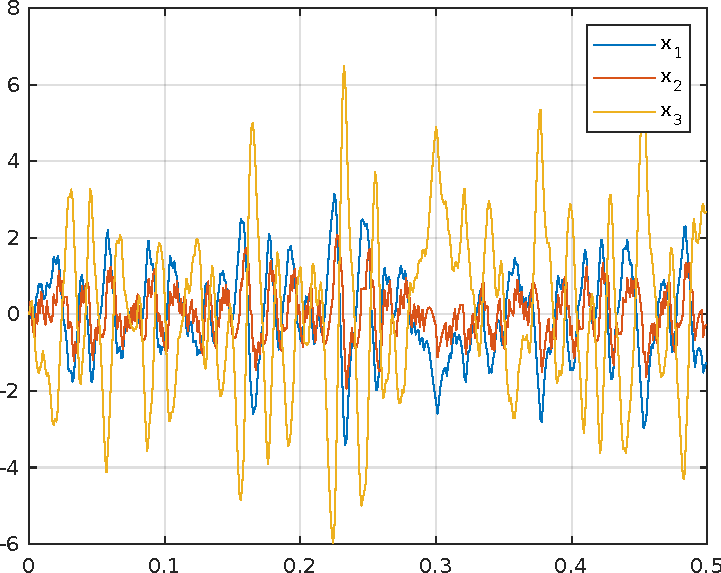
\includegraphics[width=\textwidth]{figures/ss_id_states.pdf}	
		\subcaption{States}
	\end{subfigure}
	\caption{Simulation on the identified state-space model using the input data $u$. On the left the predicted output is compared to the measured output and on the right the evolution of state variable is shown.}
	\label{fig:ss_id_results}
\end{figure}
